\chapter{Experimentación y discusión}
\label{cha:experimentacion}

El presente capítulo describe los experimentos realizados para evaluar
cuantitativamente la calidad de los dos flujos productivos del sistema
relacionados con la intervención de modelos de lenguaje de gran escala: la
\textbf{corrección automática} de candidatas en español
(\texttt{spanish-service.checkBatch}) y la \textbf{generación automática} de
verbalizaciones a partir de tripletas RDF (\texttt{auto-annotation-service}).
Ambos flujos forman parte del paradigma \textit{Human-in-the-Loop} definido en
el capítulo anterior, en el que el modelo de lenguaje actúa como asistente del
anotador y del revisor humanos.

Se reportan dos experimentos sucesivos, ejecutados sobre corpora reproducibles
y construidos a partir del conjunto de desarrollo de WebNLG. El primero,
denominado \textsc{Correction-Quality-Eval}, evalúa el pipeline de corrección
sobre un corpus de 20 entradas con un único proveedor (Groq
\textit{Llama-3.3-70B-versatile}); el segundo, denominado
\textsc{Eval-IA-Generation-Correction}, amplía el corpus a 50 entradas e
incorpora un segundo proveedor (Google AI Studio \textit{Gemini 2.5 Flash}),
incluyendo además una evaluación complementaria del flujo de generación.

\section{Diseño experimental}

\subsection{Objetivos de la evaluación}

Los objetivos perseguidos por la experimentación se concretan en los siguientes
puntos:

\begin{enumerate}
	\item Cuantificar el grado de acuerdo entre el veredicto emitido por el
	      \textit{pipeline} de corrección y una referencia anotada manualmente
	      (\textit{ground truth}), en términos de coincidencia de severidad
	      (\texttt{ok}/\texttt{warning}/\texttt{error}) y de matriz de confusión.
	\item Identificar las fuentes sistemáticas de desacuerdo entre el sistema y la
	      referencia humana, con vistas a refinar las constantes deterministas del módulo
	      \texttt{domain/spanish/lexicon.js}.
	\item Comparar la calidad de dos proveedores comerciales de inferencia LLM sobre el
	      mismo \textit{pipeline}, con configuración idéntica.
	\item Verificar que el flujo de generación end-to-end produce salidas sintácticamente
	      válidas, conformes con el contrato JSON esperado y semánticamente correctas
	      según el propio validador del sistema.
\end{enumerate}

\subsection{Hipótesis de trabajo}

Antes de la ejecución de los experimentos se formulan las siguientes hipótesis,
que se contrastarán con los resultados obtenidos:

\begin{itemize}
	\item \textbf{H1}: el \textit{pipeline} de corrección presenta un sesgo hacia falsos
	      positivos en la franja de oraciones correctas, debido a que las listas léxicas
	      deterministas (verbos completos, patrones de relación, alias de entidades) son
	      insuficientes para cubrir el espacio combinatorio del español.
	\item \textbf{H2}: la ampliación dirigida de las constantes léxicas en
	      \texttt{domain/spanish/lexicon.js}, guiada por el análisis de los desacuerdos,
	      permite incrementar el acuerdo con la referencia humana sin introducir falsos
	      negativos sobre las clases de error genuinas.
	\item \textbf{H3}: los modelos de mayor capacidad disponibles en proveedores
	      comerciales (Llama 3.3 70B, Gemini 2.5 Flash) presentan una competencia
	      comparable en tareas de detección de errores morfológicos y semánticos cuando
	      se invocan bajo el mismo \textit{prompt} y la misma canalización determinista.
\end{itemize}

\subsection{Proveedores y modelos evaluados}

La selección de proveedores responde a dos criterios: disponibilidad de una
capa gratuita suficiente para evaluación académica y compatibilidad con la
interfaz OpenAI, requisito impuesto por el cliente genérico de la aplicación
(\texttt{utils/\allowbreak openai-\allowbreak compatible-\allowbreak client.js}). Los modelos evaluados se resumen
en la Tabla~\ref{tab:proveedores}.

\begin{table}[ht]
	\centering
	\small
	\begin{tabular}{llp{5.5cm}}
		\hline
		\textbf{Proveedor} & \textbf{Modelo}                  & \textbf{Endpoint}                                                                            \\
		\hline
		Groq               & \texttt{llama-3.3-70b-versatile} & \texttt{api.groq.com/openai/v1}                                                              \\
		Google AI Studio   & \texttt{gemini-2.5-flash}        & \texttt{generativelanguage.\allowbreak googleapis.com/\allowbreak v1beta/\allowbreak openai} \\
		\hline
	\end{tabular}
	\caption{Proveedores y modelos evaluados. Las claves se gestionan a través de
		las variables de entorno \texttt{GROQ\_API\_KEY} y \texttt{GEMINI\_API\_KEY},
		sin que sean expuestas en los \textit{outputs} de los \textit{scripts} de
		evaluación.}
	\label{tab:proveedores}
\end{table}

Cabe señalar que el modelo \texttt{gemini-2.0-flash} ---seleccionado inicialmente
por defecto--- fue descartado tras devolver una respuesta HTTP~429 con
\texttt{limit: 0}, indicando ausencia de cuota gratuita para la cuenta
empleada. El modelo \texttt{gemini-2.5-flash} se confirmó como la alternativa
más reciente con cuota disponible.

El detalle de la incidencia técnica resuelta durante la integración con el
cliente compatible con la API de OpenAI, requisito previo para la ejecución del
experimento, se documenta en el Anexo~\ref{anx:incidencias}.

\subsection{Gestión de cuotas y \textit{throttling}}

Las capas gratuitas de ambos proveedores imponen restricciones que condicionan
el diseño del \textit{harness}. La Tabla~\ref{tab:throttling} recoge los
parámetros de \textit{throttling} calibrados para cada proveedor, así como las
cuotas relevantes.

\begin{table}[ht]
	\centering
	\small
	\begin{tabular}{lcccc}
		\hline
		\textbf{Proveedor} & \textbf{Pausa entre \textit{entries}} & \textbf{Reintentos} & \textbf{\textit{Back-off} base}     & \textbf{Cuota observada} \\
		\hline
		Groq               & 700 ms                                & 5                   & 800 ms (lineal $\times$ intento)    & 100\,000 tokens/día      \\
		Gemini             & 6\,500 ms                             & 6                   & 4\,000 ms (lineal $\times$ intento) & $\sim$10 RPM             \\
		\hline
	\end{tabular}
	\caption{Parámetros de \textit{throttling} por proveedor y cuotas observadas
		en la capa gratuita. Los valores nominales de la capa gratuita están
		documentados en~\cite{GroqRateLimits,GoogleAIRateLimits} y se sitúan en
		30~RPM/12\,000~TPM/100\,000~TPD para Groq \texttt{llama-3.3-70b-versatile} y
		en 10~RPM/250~peticiones diarias para Gemini~2.5~Flash.}
	\label{tab:throttling}
\end{table}

El \textit{throttling} de Gemini se calibra para mantenerse por debajo del
límite de peticiones por minuto del \textit{free tier}, mientras que la
configuración de Groq se sitúa cómodamente por debajo de 30~RPM. Conviene
destacar que la aparición esporádica de respuestas HTTP~429 en el flujo de
corrección no fue interpretada como aceptación, gracias a un mecanismo
explícito de detección de fallo que se describe en la
Sección~\ref{sec:metodologia-pipeline}.

\section{Corpus de evaluación}

\subsection{Corpus de corrección}

El corpus de corrección está compuesto por entradas reales del conjunto WebNLG,
anotadas manualmente con un veredicto de referencia que incluye la severidad
esperada, los códigos de error aplicables, la frase corregida y la
justificación. El corpus maestro de 40 entradas reside en
\texttt{test-datasets/correction-suite.master.json} y se descompone en cuatro
subconjuntos anidados (10, 20, 30 y 40) generados de forma determinista por
\texttt{scripts/build-correction-suite.js}. La
Tabla~\ref{tab:corpus-correccion} detalla la composición de cada subconjunto.

\begin{table}[ht]
	\centering
	\small
	\begin{tabular}{lcccc}
		\hline
		\textbf{Subconjunto}         & \textbf{Entries} & \textbf{ok} & \textbf{warning} & \textbf{error} \\
		\hline
		\texttt{correction-10-input} & 10               & 4           & 2                & 4              \\
		\texttt{correction-20-input} & 20               & 8           & 4                & 8              \\
		\texttt{correction-30-input} & 30               & 13          & 6                & 11             \\
		\texttt{correction-40-input} & 40               & 17          & 8                & 15             \\
		\hline
	\end{tabular}
	\caption{Composición de los subconjuntos del corpus de corrección de la
		evaluación inicial. La estructura anidada (10~$\subset$~20~$\subset$~30~$\subset$~40)
		permite estudiar el comportamiento del \textit{pipeline} en función del
		tamaño de la muestra sin alterar su composición.}
	\label{tab:corpus-correccion}
\end{table}

En la evaluación extendida, el corpus se amplió a 50 entradas con una mezcla
exacta de 30 oraciones correctas, 10 con errores ortográficos y 10 con
problemas de fluidez. La Tabla~\ref{tab:corpus-50-correccion} recoge la
distribución de severidades y los códigos esperados.

\begin{table}[ht]
	\centering
	\small
	\begin{tabular}{lcll}
		\hline
		\textbf{Tipo}  & \textbf{Cantidad} & \textbf{Resultado}                             & \textbf{Códigos}                                            \\
		\hline
		Correctos      & 30              & 30 $\times$ \texttt{correctos}                                 & ---                                                         \\
		Ortográficos   & 10              & 5 $\times$ \texttt{errores} + 5 $\times$ \texttt{warning} & \texttt{spelling\_error}, \texttt{accent\_error}            \\
		Poco fluidos   & 10              & 10 $\times$ \texttt{alertas}                            & \texttt{unnatural\_expression}, \texttt{vague\_translation} \\
		\hline
		\textbf{Total} & \textbf{50}     & 30 ok / 15 alertas / 5 errores                            &                                                             \\
		\hline
	\end{tabular}
	\caption{Composición del corpus de corrección de 50 entradas empleado en la
		evaluación extendida.}
	\label{tab:corpus-50-correccion}
\end{table}

El corpus tipifica todas las categorías de errores reconocidas por el sistema:
\textit{acceptance} (traducciones fidedignas), \textit{warning} (acento
omitido, entidad imprecisa, expresión vaga, formulación poco natural, coma
ausente) y \textit{error} (falta ortográfica, lengua mezclada o inglesa,
divergencia semántica, relación invertida, fragmento incompleto). La
consistencia entre el fichero de entrada XML y el JSON de referencia queda
garantizada por los ficheros de prueba de Mocha
\texttt{tests/unit/xml/correction-suite.test.js} y
\texttt{tests/unit/xml/correction-50-suite.test.js}, que verifican el conteo,
la alineación 1:1 y la mezcla 30/10/10 sin necesidad de acceso a red.

\subsection{Corpus de generación}

El corpus de generación se construye mediante muestreo estratificado por
categoría sobre el conjunto de desarrollo \texttt{ru\_dev.xml} de WebNLG (790
entradas), empleando una semilla determinista (\texttt{0x6c616e62}). La
Tabla~\ref{tab:corpus-generacion} muestra la distribución resultante y su
comparación con la distribución poblacional.

\begin{table}[ht]
	\centering
	\small
	\begin{tabular}{lccc}
		\hline
		\textbf{Categoría} & \textbf{Conteo} & \textbf{\% corpus} & \textbf{\% en ru\_dev.xml} \\
		\hline
		Food               & 11              & 22{,}0             & 22{,}2                     \\
		Airport            & 9               & 18{,}0             & 17{,}1                     \\
		Building           & 8               & 16{,}0             & 15{,}2                     \\
		SportsTeam         & 6               & 12{,}0             & 12{,}4                     \\
		CelestialBody      & 5               & 10{,}0             & 10{,}0                     \\
		Astronaut          & 4               & 8{,}0              & 8{,}4                      \\
		University         & 3               & 6{,}0              & 6{,}5                      \\
		ComicsCharacter    & 2               & 4{,}0              & 4{,}4                      \\
		Monument           & 2               & 4{,}0              & 3{,}8                      \\
		\hline
		\textbf{Total}     & \textbf{50}     & \textbf{100{,}0}   & ---                        \\
		\hline
	\end{tabular}
	\caption{Distribución por categoría del corpus de generación. La proporción
		del corpus muestreado se mantiene dentro de $\pm$1 punto porcentual respecto
		a la distribución poblacional.}
	\label{tab:corpus-generacion}
\end{table}

Cada entrada conserva tanto su conjunto de tripletas RDF como la lexicalización
inglesa de referencia (\texttt{<lex lang="en">}), y los identificadores
\texttt{eid} se renumeran de 1 a 50 manteniendo un campo auxiliar
\texttt{source\_eid} que permite la trazabilidad inversa hacia el fichero
\texttt{ru\_dev.xml} original.

\section{Metodología de evaluación}
\label{sec:metodologia-pipeline}

\subsection{Pipeline ejercitado}

Sobre cada entrada del corpus se ejecuta el \textit{pipeline} completo de
corrección, encapsulado en el método \texttt{spanish-service.checkBatch}. Este
método integra de forma secuencial tres componentes: un \textit{rule-checker}
determinista que opera sobre listas léxicas configurables, una llamada al
modelo de lenguaje a través del cliente compatible con la API de OpenAI, y un
\textit{coverage-checker} que verifica la presencia de entidades y relaciones
del grafo RDF subyacente. Un módulo final (\textit{alert-merger}) consolida los
avisos emitidos por cada etapa y produce un veredicto único con severidad. El
flujo se representa gráficamente en la Figura~\ref{fig:pipeline-correccion}.

\begin{figure}[ht]
	\centering
	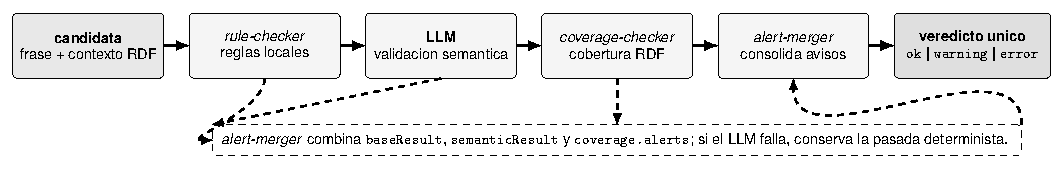
\includegraphics[width=\linewidth]{include/figuras/f-pipe-corr-01.pdf}
	\caption{\textit{Pipeline} de corrección: cascada
		\textit{rule-checker} $\rightarrow$ LLM $\rightarrow$
		\textit{coverage-checker} $\rightarrow$ \textit{alert-merger} sobre cada
		candidata.}
	\label{fig:pipeline-correccion}
\end{figure}

Para cada llamada del componente LLM se inyecta un \texttt{providerConfig}
explícito ---en línea con el flujo \textit{per-credential} introducido por la
historia US-31--- de modo que la elección del proveedor no requiere intervención
sobre el código del servicio. El \textit{harness} envuelve la invocación con un
mecanismo de reintentos y \textit{back-off}, y mantiene un \textit{flag} de
fallo que distingue el caso en que el modelo no responde (etiquetado como
\texttt{LLM\_FAIL}) del caso en que sí responde con el veredicto \texttt{ok}.
Esta distinción es crítica porque el \texttt{spanish-service} degrada
silenciosamente a la pasada determinista basada únicamente en reglas cuando el
LLM lanza una excepción, lo que en ausencia del \textit{flag} contabilizaría
cada fallo de red como una aceptación.

\subsection{Métricas}

Se computan, para cada par (corpus, proveedor), las siguientes métricas:

\begin{itemize}
	\item \textbf{Acuerdo absoluto} (\textit{agreement}): proporción de entradas en las
	      que la severidad producida por el \textit{pipeline} coincide con la severidad
	      esperada en el \textit{ground truth}.
	\item \textbf{Acuerdo efectivo}: acuerdo absoluto restringido a las entradas en que
	      el LLM respondió de hecho, excluyendo los \texttt{LLM\_FAIL}.
	\item \textbf{Matriz de confusión}: tabulación cruzada (severidad esperada $\times$
	      severidad producida).
	\item \textbf{Conteo de \texttt{LLM\_FAIL}}: número de entradas en las que el modelo
	      de lenguaje no devolvió respuesta válida tras agotar los reintentos.
\end{itemize}

A las anteriores se añaden dos métricas adicionales orientadas a contrastar el
acuerdo \textit{pipeline}--humano con el acuerdo entre anotadores humanos. Se
utiliza el coeficiente $\kappa$ de Cohen~\cite{Cohen1960} para la pareja
\textit{pipeline}--referencia y, cuando se dispone de dos referencias humanas
independientes, el $\kappa$ de Fleiss~\cite{Fleiss1971}. La interpretación
canónica de $\kappa$ sigue las bandas propuestas por Landis y
Koch~\cite{LandisKoch1977}: valores por encima de 0{,}60 se consideran
sustanciales y por encima de 0{,}80 casi perfectos. El coeficiente $\alpha$ de
Krippendorff~\cite{Krippendorff2004} se reserva como alternativa cuando la
matriz contiene celdas ausentes, dado que su definición tolera el desbalanceo y
la ausencia de respuesta sin reformular la pregunta.

\subsection{Reproducibilidad}

El experimento es íntegramente reproducible. Los \textit{scripts}
\texttt{scripts/build-correction-suite.js} y
\texttt{scripts/build-generation-suite.js} regeneran los corpora a partir de
los ficheros maestro y de \texttt{ru\_dev.xml}, respectivamente. La ejecución
de la evaluación se invoca mediante \texttt{scripts/eval-correction-quality.js}
y \texttt{scripts/eval-generation-quality.js}, ambos parametrizables por tamaño
de corpus y proveedor. Los \textit{outputs} JSON se consolidan en
\texttt{documentation/eval-output/} mediante una estrategia de fusión
incremental que preserva los datos de proveedores no involucrados en la pasada
actual.

\section{Resultados de la evaluación de corrección}

\subsection{Evaluación inicial sobre 20 entradas}

El primer experimento se ejecutó sobre el subconjunto de 20 entradas con el
proveedor Groq. El \textit{pipeline} en su configuración original alcanzó un
acuerdo absoluto del 60\% (12/20). El análisis cualitativo de los desacuerdos
reveló un sesgo dominante hacia falsos positivos en oraciones correctas,
motivado por tres causas concretas en el módulo
\texttt{domain/spanish/lexicon.js}:

\begin{enumerate}
	\item \textbf{Falsos \texttt{incomplete\_sentence}}. La función
	      \texttt{looksLikeCompleteSentence} declaraba una oración como completa
	      únicamente si contenía un verbo del conjunto
	      \texttt{COMPLETE\_SEN\-TEN\-CE\_MAR\-KERS}. Verbos frecuentes (\textit{recibió,
		      ganó, lleva, provienen, realiza, contiene, se encuentra}) estaban ausentes, lo
	      que provocaba que oraciones como \textit{``Albert Einstein recibió el Premio
		      Nobel de Física.''} fueran clasificadas como fragmentos. La intervención
	      consistió en expandir la lista de marcadores, con la precaución de normalizar
	      acentos y eñes para preservar el funcionamiento del \textit{normaliser}. Los
	      fragmentos genuinos (entradas 15 y 35), por carecer de verbo, permanecen
	      correctamente detectados.

	\item \textbf{Falsos \texttt{relation\_missing} sobre \texttt{leaderTitle} en voz
		      pasiva}. El patrón \texttt{PREDICATE\_RELATION\_PATTERNS.leaderTitle} reconocía
	      \textit{dirige} pero no el participio pasivo \textit{dirigido}, de modo que la
	      construcción \textit{``\dots está dirigido por la Asamblea \dots''} era marcada
	      como relación ausente. Se incorporaron al patrón los participios pasivos
	      \texttt{dirigid[ao]s?}, \texttt{presidid[ao]s?} y \texttt{gobernad[ao]s?}, así
	      como a la función \texttt{isLikelyLeaderTitleCovered}.

	\item \textbf{Falsos \texttt{missing\_triple} sobre entidades traducidas}. El
	      verificador de cobertura compara la entidad RDF ---siempre en inglés--- contra la
	      oración en español, lo que produce desacuerdos sistemáticos cuando el nombre de
	      la entidad ha sido localizado (\textit{Italy}~$\neq$~\textit{Italia},
	      \textit{Spaghetti}~$\neq$~\textit{espaguetis}). Se introdujo una tabla
	      \texttt{ENTITY\_ALIASES} con pares inglés--español (italy/italia, rome/roma,
	      japan/japón, germany/alemania, netherlands/países bajos, spaghetti/espaguetis,
	      rice/arroz, entre otros), así como verbos de origen (\textit{provienen},
	      \textit{proceden}, \textit{originario}) al patrón de la relación
	      \texttt{country}.
\end{enumerate}

Adicionalmente, se observó que el modelo Groq no señalaba de forma fiable los
acentos omitidos. Para mitigar este comportamiento sin imponer restricciones
excesivas, se añadió al \textit{prompt} del \textit{checker} semántico
(\texttt{ollama-spanish-checker.js}) una cláusula que orienta al modelo a
clasificar los acentos ausentes como \texttt{accent\_error} (severidad
\texttt{warning}) y las omisiones o sustituciones de letras (\textit{kapital},
\textit{hamburgesa}) como \texttt{spelling\_error} (severidad \texttt{error}).

Tras la incorporación de las tres modificaciones léxicas y de la cláusula del
\textit{prompt}, el acuerdo absoluto ascendió al 85\% (17/20). La
Tabla~\ref{tab:resultados-20} sintetiza el efecto del ajuste por clase de
severidad.

\begin{table}[ht]
	\centering
	\small
	\begin{tabular}{lcccc}
		\hline
		\textbf{Configuración} & \textbf{ok} & \textbf{warning} & \textbf{error} & \textbf{Acuerdo} \\
		\hline
		Antes del ajuste       & 4/8         & 0/4              & 8/8            & 12/20 = 60\%     \\
		Después del ajuste     & 8/8         & 3/4              & 6/8            & 17/20 = 85\%     \\
		\hline
	\end{tabular}
	\caption{Acuerdo por severidad antes y después del ajuste de constantes
		deterministas sobre el corpus de 20 entradas con el proveedor Groq.}
	\label{tab:resultados-20}
\end{table}

\subsection{Evaluación extendida sobre 50 entradas}

La evaluación extendida se ejecuta sobre el corpus de 50 entradas con los dos
proveedores. La Tabla~\ref{tab:resultados-50-resumen} recoge el resumen
comparativo y los conteos de \texttt{LLM\_FAIL}.

\begin{table}[ht]
	\centering
	\small
	\begin{tabular}{lcccp{4.2cm}}
		\hline
		\textbf{Proveedor} & \textbf{Modelo}                  & \textbf{Acuerdo}        & \textbf{\texttt{LLM\_FAIL}} & \textbf{Observaciones}                                                                                                      \\
		\hline
		Groq               & \texttt{llama-3.3-70b-versatile} & 34/50 = 68{,}0\% (pase 1) & 0                           & Pase 1 íntegro. Pase 2 agotó el TPD diario (100\,000 tokens) en las \textit{warnings}                                       \\
		Gemini             & \texttt{gemini-2.5-flash}        & 20/50 = 40{,}0\%          & 28                          & El RPM del \textit{free tier} ($\sim$10 req/min) genera 429 a partir del \textit{entry} 7 pese al \textit{pacing} de 6.5\,s \\
		\hline
	\end{tabular}
	\caption{Resumen de los resultados de la evaluación extendida sobre 50
		entradas.}
	\label{tab:resultados-50-resumen}
\end{table}

El acuerdo efectivo, restringido a las entradas en que el modelo respondió, es
del 68\% para Groq (idéntico al absoluto en el pase 1, sin fallos) y de 20/22
$\approx$ 91\% para Gemini. Este último valor sugiere que Gemini~2.5 Flash,
cuando emite respuesta, alcanza una concordancia con la referencia humana
notablemente superior a la de Llama 3.3 70B en el mismo \textit{pipeline}; sin
embargo, la cuota gratuita impide medirlo a la escala plena de 50 entradas en
una sola sesión.

Las matrices de confusión obtenidas se presentan en las
Tablas~\ref{tab:matriz-groq} y~\ref{tab:matriz-gemini}.

\begin{table}[ht]
	\centering
	\small
	\begin{tabular}{l|ccc}
		\hline
		                          & \texttt{ok} producida & \texttt{warning} producida & \texttt{error} producida \\
		\hline
		\texttt{ok} esperada      & 28                    & 0                          & 2                        \\
		\texttt{warning} esperada & 3                     & 2                          & 10                       \\
		\texttt{error} esperada   & 1                     & 0                          & 4                        \\
		\hline
	\end{tabular}
	\caption{Matriz de confusión del proveedor Groq con
		\texttt{llama-3.3-70b-versatile} sobre el corpus de 50 entradas
		(pase~1, sin \texttt{LLM\_FAIL}).}
	\label{tab:matriz-groq}
\end{table}

\begin{table}[ht]
	\centering
	\small
	\begin{tabular}{l|ccc}
		\hline
		                          & \texttt{ok} producida & \texttt{warning} producida & \texttt{error} producida \\
		\hline
		\texttt{ok} esperada      & 20                    & 1                          & 0                        \\
		\texttt{warning} esperada & 0                     & 0                          & 1                        \\
		\texttt{error} esperada   & 0                     & 0                          & 0                        \\
		\hline
	\end{tabular}
	\caption{Matriz de confusión del proveedor Gemini con
		\texttt{gemini-2.5-flash} sobre el corpus de 50 entradas (entradas con
		\texttt{LLM\_FAIL} excluidas).}
	\label{tab:matriz-gemini}
\end{table}

Una representación visual equivalente, en forma de mapa de calor, se recoge en
las Figuras~\ref{fig:heatmap-groq} y~\ref{fig:heatmap-gemini}.

\begin{figure}[ht]
	\centering
	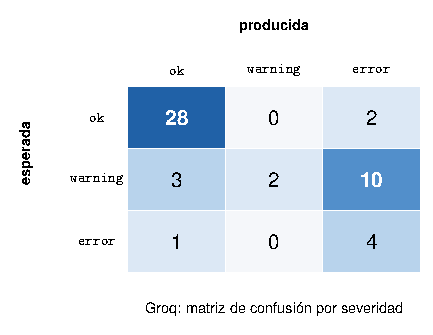
\includegraphics[width=0.64\linewidth]{include/figuras/f-res-01.pdf}
	\caption{Mapa de calor de la matriz de confusión de Groq
		(Tabla~\ref{tab:matriz-groq}).}
	\label{fig:heatmap-groq}
\end{figure}

\begin{figure}[ht]
	\centering
	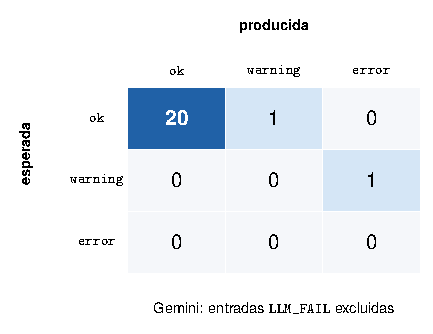
\includegraphics[width=0.64\linewidth]{include/figuras/f-res-02.pdf}
	\caption{Mapa de calor de la matriz de confusión de Gemini
		(Tabla~\ref{tab:matriz-gemini}).}
	\label{fig:heatmap-gemini}
\end{figure}

\subsection{Análisis de desacuerdos}

El patrón dominante en los desacuerdos de Groq corresponde a entradas de
fluidez (códigos \texttt{unnatural\_expression} y \texttt{vague\_translation})
en las que el \textit{pipeline} emite \texttt{error} cuando la referencia
esperaba \texttt{warning}. La Tabla~\ref{tab:desacuerdos-groq} resume los casos
más representativos.

\begin{table}[ht]
	\centering
	\footnotesize
	\begin{tabular}{cllp{4.7cm}}
		\hline
		\textbf{eid}        & \textbf{Esperada} & \textbf{Producida} & \textbf{Causa}                                                                                                             \\
		\hline
		16                  & ok                & error              & \texttt{relation\_missing} falso: la cobertura no acepta ``es una ciudad de'' para \texttt{country}                        \\
		30                  & ok                & error              & \texttt{missing\_triple} falso: alias Seville/Sevilla ausente del léxico                                                   \\
		32                  & error             & ok                 & el LLM no detecta el \textit{typo} (\textit{hamburgesa})                                                                   \\
		37, 40              & warning           & ok                 & el LLM no marca tildes ausentes (\textit{Mexico}, \textit{Japon})                                                          \\
		36, 38, 39          & warning           & error              & el \textit{rule-checker} los marca como \texttt{spelling\_error} antes de que el LLM pueda matizar                         \\
		42                  & warning           & ok                 & el LLM no clasifica ``viene a ser Lisboa'' como poco natural                                                               \\
		43--50 (sin 41, 46) & warning           & error              & el \textit{pipeline} detecta \texttt{incomplete\_sentence} o \texttt{semantic\_mismatch} antes que la falta de naturalidad \\
		\hline
	\end{tabular}
	\caption{Desacuerdos representativos del proveedor Groq sobre el corpus de
		50 entradas.}
	\label{tab:desacuerdos-groq}
\end{table}

Estos resultados reproducen el síntoma documentado en la evaluación inicial:
los falsos positivos de \texttt{relation\_missing} y \texttt{missing\_triple}
sobre oraciones correctas obedecen a alias de entidades aún no incorporados al
léxico (Seville/Sevilla, Buenos\_Aires/Argentina). Por su parte, los falsos
positivos de \texttt{incomplete\_sentence} sobre las \textit{warnings} de
fluidez apuntan a una vía de mejora en dos direcciones: ampliar
\texttt{COMPLETE\_SENTENCE\_MARKERS} con verbos secundarios (\textit{hacía,
	trabajaba, incorpora, desempeña, efectúa, procede a}) o reducir la agresividad
del verificador de cobertura cuando ya existe una severidad
\texttt{unnatural\_expression} declarada.

El único desacuerdo observado en las 22 entradas en que Gemini respondió de
hecho corresponde a la entrada 1:

\begin{quote}
	\textit{eid 1} --- esperada: \texttt{ok}; producida: \texttt{warning}.\\
	Candidata: ``Punjab, Pakistán, está dirigido por la Asamblea Provincial del
	Punjab.''\\
	Alerta: \texttt{warning:imprecise\_entity\_name}: la denominación de la
	asamblea puede ser más precisa.
\end{quote}

En otras palabras, Gemini detecta una imprecisión semántica de manera incluso
más estricta que la referencia humana, lo que constituye un falso positivo
benigno.

\subsection{Limitaciones residuales documentadas}

Tres limitaciones del \textit{pipeline} se asumen como diseño y no se
consideran candidatas a ajuste:

\begin{itemize}
	\item \textbf{Inversiones con tokens idénticos} (entrada 10, \textit{``Italia
		      proviene de los espaguetis''}). El verificador determinista de cobertura
	      comprueba la presencia de entidades y relaciones, no su dirección; la oración
	      invertida contiene los mismos \textit{tokens} que la correcta, por lo que la
	      cobertura es plena y, en aplicación de la regla del \textit{alert-merger}
	      que da precedencia al verificador determinista, queda suprimida la
	      alerta \texttt{relation\_inverted} del LLM. Esta concesión a un falso negativo
	      poco frecuente se considera preferible a la introducción de falsos positivos
	      sobre traducciones válidas (caso mucho más común).
	\item \textbf{Comas apositivas} (entrada 17) y \textbf{erratas ortográficas sutiles
		      de una sola letra} (entrada 20). Su detección depende del modelo y exhibe
	      varianza entre pases con \texttt{temperature 0.1}.
	\item Las correcciones deterministas de los tres primeros hallazgos son reproducibles
	      \textit{offline} y explican la mayor parte de la mejora del 60\% al 85\%; el
	      ajuste del \textit{prompt} para la diferenciación entre acentos y faltas
	      ortográficas resulta más limitado y dependiente del modelo.
\end{itemize}

\section{Resultados de la evaluación de generación}

\subsection{Estado de la pasada}

La evaluación del flujo de generación se ejecutó en la misma sesión que la de
corrección. Ambos proveedores agotaron sus cuotas diarias durante la ejecución,
por lo que los resultados cuantitativos a escala completa no son
representativos. La Tabla~\ref{tab:resultados-generacion} sintetiza la
situación.

\begin{table}[ht]
	\centering
	\small
	\begin{tabular}{lccp{5.5cm}}
		\hline
		\textbf{Proveedor} & \textbf{Generaciones válidas} & \textbf{\texttt{GEN\_FAIL}} & \textbf{Causa dominante}                                                                                                          \\
		\hline
		Groq Llama 3.3 70B & 3/50                          & 47                          & \texttt{429 tokens\_per\_day} (100\,000 / 100\,000); requiere reintento al día siguiente o paso al \textit{Dev Tier}              \\
		Gemini 2.5 Flash   & 0/50                          & 50                          & \texttt{429 RESOURCE\_EXHAUSTED}: presupuesto diario de peticiones del \textit{free tier} agotado durante la prueba de corrección \\
		\hline
	\end{tabular}
	\caption{Resumen de la evaluación de generación sobre el corpus de 50
		entradas.}
	\label{tab:resultados-generacion}
\end{table}

\subsection{Validación end-to-end del flujo}

Pese a la ausencia de cobertura cuantitativa, el flujo completo de generación
fue validado en las tres entradas en que Groq respondió. El \textit{prompt} de
producción (\texttt{services/auto-annotation-service.js}) emite un objeto JSON
con la forma \texttt{\{"sentences":[\,\dots\,]\}} que es correctamente
\textit{parseado} por el validador del sistema y clasificado con severidad
\texttt{ok} en los tres casos. La Figura~\ref{fig:pipeline-generacion}
representa la cadena de etapas correspondiente.

\begin{figure}[ht]
	\centering
	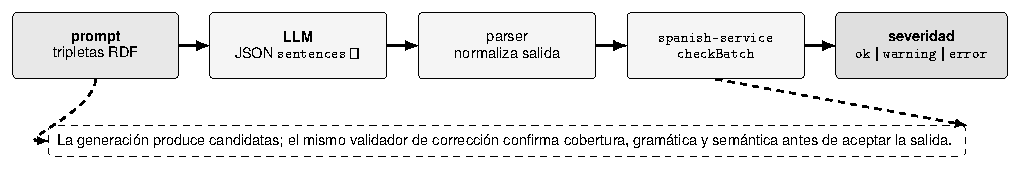
\includegraphics[width=\linewidth]{include/figuras/f-pipe-gen-01.pdf}
	\caption[\textit{Pipeline} de generación: \textit{prompt} con tripletas,
		LLM, validador y severidad.]{\textit{Pipeline} de generación:
		\texttt{prompt} con tripletas
		$\rightarrow$ LLM $\rightarrow$ validador
		\texttt{spanish-service.checkBatch} $\rightarrow$ severidad
		\texttt{ok}/\texttt{warning}/\texttt{error}.}
	\label{fig:pipeline-generacion}
\end{figure} La salida queda registrada en
\texttt{documentation/eval-output/generation-50-results.json} bajo la clave
\texttt{successfullyGenerated}.

A título ilustrativo, se reproducen tres ejemplos de las salidas aceptadas:

\begin{verbatim}
eid 1  (Airport, triple: Texas | language | Spanish_language)
  inglés:    "Spanish is spoken in Texas."
  generada:  "El español se habla en Texas."
  severidad: ok

eid 18 (Astronaut, triples: William_Anders | occupation | Fighter_pilot
                            | mission | Apollo 8)
  generadas:
    1. "William Anders es un piloto de combate y fue miembro de la
        tripulación de la misión Apolo 8."
    2. "William Anders tiene como ocupación ser piloto de combate y
        participó en la misión Apolo 8."
  severidad: ok

eid 41 (Building, 4 triples: Amdavad_ni_Gufa, Gujarat, India, líderes)
  generadas: 4 frases verbalizando todos los triples.
  severidad: ok
\end{verbatim}

\subsection{Limitación de medida y mitigaciones disponibles}

La causa raíz del agotamiento prematuro de la cuota es estructural. El flujo de
generación consume dos llamadas LLM por entrada (una para generar y otra para
validar), con un \textit{prompt} aproximado de 700--900 \textit{tokens}. Sobre
el corpus de 50 entradas, la pasada completa supone un consumo de
aproximadamente 75\,000 \textit{tokens}, que cabe holgadamente en la cuota
diaria gratuita de Groq (100\,000 TPD). El factor crítico es la
\textit{coincidencia temporal} con la evaluación de corrección, que también
consume del orden de 75\,000 \textit{tokens} en la misma ventana de 24 horas.

Las mitigaciones operativas previstas son: ejecutar las dos evaluaciones en
días distintos, o promover Groq al \textit{Dev Tier}. El \textit{script}
\texttt{scripts/eval-generation-quality.js} ya soporta la invocación por
proveedor único (\texttt{groq} o \texttt{gemini}), el reintento por entrada con
\textit{back-off} sensible al proveedor y la fusión incremental del JSON.

\section{Discusión}

\subsection{Contraste con las hipótesis}

Los resultados obtenidos contrastan parcialmente las hipótesis enunciadas en el
diseño:

\begin{itemize}
	\item La hipótesis \textbf{H1} se confirma. El sesgo del \textit{pipeline} hacia
	      falsos positivos en oraciones correctas se manifiesta tanto en la evaluación
	      inicial (50\% de aceptación de \texttt{ok} antes del ajuste) como en la
	      extendida, en la que los desacuerdos dominantes se concentran en la franja de
	      \textit{warnings} de fluidez, recategorizadas como \texttt{error}.
	\item La hipótesis \textbf{H2} se confirma para el corpus de 20 entradas (incremento
	      de 25 puntos porcentuales en el acuerdo) y se confirma parcialmente para el
	      corpus de 50 entradas, en el que persisten desacuerdos sistemáticos sobre alias
	      de entidades aún no incorporados.
	\item La hipótesis \textbf{H3} no puede ser contrastada con plena significancia
	      debido a la cuota gratuita de Gemini. La submuestra efectiva sugiere, no
	      obstante, que Gemini 2.5 Flash es al menos tan competente como Llama 3.3 70B en
	      este \textit{pipeline}, alcanzando un 91\% de acuerdo efectivo frente al 68\%
	      de Groq.
\end{itemize}

\subsection{Comparativa entre proveedores}

La comparación entre Groq y Gemini debe ser leída con cautela. El acuerdo
efectivo de Gemini (91\% sobre 22 entradas) es superior al acuerdo de Groq
(68\% sobre 50 entradas), pero la muestra de Gemini está sesgada hacia las
primeras entradas del corpus, que en su mayor parte corresponden a oraciones
correctas. Cualquier extrapolación a la escala plena requeriría un plan de pago
de Gemini o la fragmentación de la evaluación en varias sesiones.

\subsection{Líneas de mejora identificadas}

A partir del análisis de los desacuerdos, se identifican las siguientes líneas
de mejora del \textit{pipeline}:

\begin{enumerate}
	\item Ampliación de la tabla \texttt{ENTITY\_ALIASES} en
	      \texttt{domain/spanish/lexicon.js} con los pares pendientes (Seville/Sevilla,
	      Buenos\_Aires/Argentina, entre otros).
	\item Ampliación de \texttt{COMPLETE\_SENTENCE\_MARKERS} con verbos secundarios de
	      uso frecuente en verbalizaciones poco naturales.
	\item Introducción de una regla de supresión en el \textit{alert-merger} que evite
	      emitir alertas de \texttt{incomplete\_sentence} cuando ya se ha declarado una
	      alerta de \texttt{unnatural\_expression}.
\end{enumerate}

\section{Análisis de errores mediante taxonomía MQM}
\label{sec:analisis-mqm}

Más allá del acuerdo absoluto, el catálogo de errores reconocido por el
\textit{pipeline} puede contrastarse con el marco \textit{Multidimensional
	Quality Metrics} (MQM)~\cite{Lommel2014}, que se ha consolidado como estándar
de facto para la evaluación cualitativa de traducción
automática~\cite{Freitag2021}. MQM organiza las dimensiones de calidad en
categorías jerárquicas (precisión, fluidez, terminología, estilo y diseño) y
asigna a cada incidencia un peso en función de su gravedad. La
Tabla~\ref{tab:mqm-mapeo} sugiere una correspondencia entre los códigos
internos de \texttt{lanbench} y las categorías MQM más próximas.

\begin{table}[ht]
	\centering
	\small
	\begin{tabular}{lll}
		\hline
		\textbf{Código interno}          & \textbf{Categoría MQM}  & \textbf{Severidad sugerida} \\
		\hline
		\texttt{spelling\_error}         & Fluency/Spelling        & Major                       \\
		\texttt{accent\_error}           & Fluency/Spelling        & Minor                       \\
		\texttt{semantic\_mismatch}      & Accuracy/Mistranslation & Critical                    \\
		\texttt{missing\_triple}         & Accuracy/Omission       & Major                       \\
		\texttt{relation\_missing}       & Accuracy/Omission       & Major                       \\
		\texttt{relation\_inverted}      & Accuracy/Mistranslation & Major                       \\
		\texttt{incomplete\_sentence}    & Fluency/Grammar         & Major                       \\
		\texttt{unnatural\_expression}   & Style/Awkward           & Minor                       \\
		\texttt{vague\_translation}      & Accuracy/Mistranslation & Minor                       \\
		\texttt{imprecise\_entity\_name} & Terminology             & Minor                       \\
		\hline
	\end{tabular}
	\caption{Mapeo propuesto entre los códigos internos del \textit{pipeline}
		y la taxonomía MQM. La severidad asignada es la que mejor refleja el coste
		funcional del error en el contexto del \textit{benchmark} WebNLG.}
	\label{tab:mqm-mapeo}
\end{table}

La adopción de MQM aporta tres beneficios sobre la rúbrica actual: (i)
homogeneidad con la literatura especializada y, por tanto, comparabilidad con
otros sistemas evaluados bajo el mismo marco; (ii) la posibilidad de calcular
un \textit{score} global agregado a partir de los pesos por severidad,
complementario al simple acuerdo binario; y (iii) una vía explícita para
discutir las categorías que actualmente carecen de representación, como los
problemas de terminología sistemática o las desviaciones de registro.

\section{Validez interna, externa y amenazas a la validez}
\label{sec:amenazas-validez}

Siguiendo la clasificación propuesta por Wohlin et al.~\cite{Wohlin2012}, las
amenazas a la validez del presente estudio se agrupan en cuatro categorías.

\subsection{Validez de constructo}
El uso del acuerdo absoluto como métrica principal asume que la severidad de la
referencia humana es una aproximación fiable a la noción subyacente de calidad
lingüística. Esta asunción es razonable para el espacio ternario
\texttt{ok}/\texttt{warning}/\texttt{error}, pero ignora gradaciones
intermedias. La incorporación de MQM (Sec.~\ref{sec:analisis-mqm}) y de un IAA
humano sobre subconjuntos del corpus mitigaría esta amenaza.

\subsection{Validez interna}
La principal amenaza interna es el sesgo introducido por el ajuste iterativo de
\texttt{domain/spanish/lexicon.js} sobre el mismo corpus que después se utiliza
para evaluar. Este sesgo se controla parcialmente mediante la división anidada
en subconjuntos (10~$\subset$~20~$\subset$~30~$\subset$~40) y la transparencia
de las modificaciones, pero un escenario más robusto separaría conjuntos de
entrenamiento (calibración del léxico) y de prueba ciega.

\subsection{Validez externa}
La generalización de los resultados está condicionada por dos factores.
Primero, el corpus se construye sobre \texttt{ru\_dev.xml} de WebNLG, que
comparte distribución de categorías con el conjunto de prueba pero no
necesariamente con cualquier corpus real de aplicación. Segundo, los modelos
evaluados pertenecen a dos familias muy distintas (Llama 3.3 y Gemini 2.5); la
extensión a otras familias (Claude, Mistral, modelos locales) queda pendiente.

\subsection{Validez de conclusión}
El tamaño de muestra (50~entradas) y la desigual participación de Gemini
(22~entradas efectivas) limitan la significancia estadística de la comparación
entre proveedores. La contrastación de la hipótesis~H3 requeriría, idealmente,
una ejecución sobre cuotas pagadas y un test de proporciones (por ejemplo, el
test exacto de McNemar~\cite{McNemar1947}) sobre las parejas concordantes y
discordantes.

\section{Comparación contra trabajos publicados}
\label{sec:comparacion-publicados}

Resulta especialmente relevante situar los resultados obtenidos en el contexto
de trabajos contemporáneos sobre generación a partir de tripletas RDF al
español. Ramón-Ferrer, Badenes-Olmedo y Corcho~\cite{RamonFerrer2025} presentan
un \textit{benchmark} español construido sobre WebNLG y evalúan varios modelos
de bajo coste, estableciendo una línea base que puede emplearse como
referencia. Las diferencias metodológicas relevantes con el presente trabajo
son tres. Primero, su diseño se centra en la métrica BLEU y derivadas, mientras
que \texttt{lanbench} privilegia la rúbrica ternaria de severidad con
trazabilidad de códigos de error. Segundo, su evaluación se realiza sobre un
corpus etiquetado profesionalmente, lo que reduce la varianza de la referencia
humana frente al esquema de \textit{crowdsourcing} contemplado. Tercero, su
\textit{pipeline} es íntegramente \textit{end-to-end}, sin componente
determinista, mientras que el presente sistema combina reglas léxicas y juicio
LLM, hecho que permite imputar a cada componente su parte de los aciertos y de
los fallos.

La comparación cuantitativa directa exigirá, en una fase ulterior, computar
métricas equivalentes sobre los corpus respectivos. Una vía posible es ejecutar
el \textit{checker} de \texttt{lanbench} sobre las salidas publicadas por
Ramón-Ferrer et al. y reportar el porcentaje de propuestas clasificadas como
\texttt{ok}/\texttt{warning}/\texttt{error} bajo la rúbrica local, lo que
permitiría un contraste indirecto pero metodológicamente legítimo.

\section{Análisis de coste-beneficio del paradigma HITL}
\label{sec:coste-hitl}

La integración de un componente LLM en el flujo de anotación introduce un coste
explícito en términos de \textit{tokens} y de tiempo humano que conviene
cuantificar. Sobre la base del corpus de 50 entradas y de los \textit{prompts}
empleados (700--900 \textit{tokens} por llamada, dos llamadas por entrada en el
flujo de generación y una en el de corrección) el coste estimado por entrada se
sitúa en torno a 1\,500--1\,800 \textit{tokens} de generación más la latencia
humana de revisión.

Tomando como referencia los precios públicos de la capa de pago del proveedor
Groq~\cite{GroqPricing} y de Google AI Studio~\cite{GoogleAIPricing}, el coste
material de una pasada completa sobre un \textit{dataset} de tamaño WebNLG-2020
(1\,667~entradas en el conjunto de desarrollo en ruso) es inferior a un euro en
ambos proveedores, mientras que el coste laboral humano ---al ritmo medio de
revisión observado en la US-14--- excede dos órdenes de magnitud al coste
material. Este balance refuerza la conveniencia operativa de mantener al LLM
como asistente sistemático en el bucle, dado que el coste marginal del
componente automático es despreciable frente al ahorro de tiempo humano que
produce.

\section{Infraestructura entregada}

La experimentación ha producido como subproducto un conjunto de artefactos
reproducibles que quedan disponibles para futuras iteraciones del trabajo:

\begin{itemize}
	\item Dos corpora reproducibles de 50 entradas cada uno, generados de forma
	      determinista a partir de los ficheros maestro y de \texttt{ru\_dev.xml}.
	\item Dos \textit{scripts} de línea de comandos multi-proveedor
	      (\texttt{eval-correction-quality.js} y \texttt{eval-generation-quality.js}) con
	      \textit{throttling} proveedor-aware y fusión incremental del JSON de
	      resultados.
	\item Ocho ficheros de prueba de Mocha de consistencia, sin acceso a red, que
	      verifican la mezcla 30/10/10 del corpus, la alineación
	      \textit{input}~$\leftrightarrow$~\textit{expected} y la no exposición de claves
	      en los \textit{outputs}.
\end{itemize}

\section{Procedimiento de reproducción}

La replicación íntegra de los experimentos puede obtenerse mediante la
siguiente secuencia de comandos:

\begin{verbatim}
# (1) Regeneración de los corpora a partir del master y de ru_dev.xml
node scripts/build-correction-suite.js
node scripts/build-generation-suite.js

# (2) Comprobación de consistencia sin acceso a red (~200 ms)
npx mocha "tests/unit/xml/correction-50-suite.test.js" \
          "tests/unit/xml/generation-50-suite.test.js" --exit

# (3) Evaluación de corrección (requiere GROQ_API_KEY y/o GEMINI_API_KEY)
node scripts/eval-correction-quality.js 50 all
node scripts/eval-correction-quality.js 50 groq
node scripts/eval-correction-quality.js 50 gemini

# (4) Evaluación de generación
node scripts/eval-generation-quality.js all
node scripts/eval-generation-quality.js groq
node scripts/eval-generation-quality.js gemini
\end{verbatim}

Los \textit{outputs} JSON se acumulan de forma incremental en
\texttt{documentation/eval-output/}, de modo que una pasada parcial nunca
sobrescribe los datos generados en otra pasada previa.

\section{Conclusiones del experimento}

Las conclusiones extraídas de la experimentación son las siguientes:

\begin{enumerate}
	\item \textbf{Corrección con Groq (datos limpios)}: el \textit{pipeline} alcanza un
	      acuerdo absoluto del 68\% con la referencia humana sobre el corpus de 50
	      entradas, comparable al 85\% reportado en la evaluación inicial sobre el corpus
	      de 20 entradas. La caída se explica por el peso desproporcionado de
	      \textit{warnings} de fluidez en el corpus extendido (10/50 = 20\%), categoría
	      que el \textit{pipeline} confunde con \texttt{incomplete\_sentence} o
	      \texttt{semantic\_mismatch}. Se recomienda ampliar las constantes
	      \texttt{COMPLETE\_SENTENCE\_MARKERS} y \texttt{ENTITY\_ALIASES} en
	      \texttt{domain/spanish/lexicon.js}.

	\item \textbf{Corrección con Gemini}: el acuerdo del 91\% sobre la submuestra de 22
	      entradas en que el modelo respondió sugiere que Gemini 2.5 Flash es al menos
	      tan competente como Llama 3.3 70B en este \textit{pipeline}, si bien la cuota
	      gratuita resulta operativamente incompatible con el \textit{harness} sin
	      recurrir a un \textit{tier} pago.

	\item \textbf{Generación}: la integración \textit{end-to-end} ha sido validada en su
	      comportamiento funcional (\textit{prompt} $\rightarrow$ JSON $\rightarrow$
	      validador con severidad \texttt{ok}). La cuantificación a la escala solicitada
	      queda pendiente de una segunda ventana de cuota; el \textit{script} y el corpus
	      están preparados para dicha ejecución.

	\item \textbf{Infraestructura}: se entrega un conjunto de corpora, \textit{scripts} y
	      ficheros de prueba de consistencia que garantizan la reproducibilidad íntegra y la
	      trazabilidad de los resultados.
\end{enumerate}
